\documentclass[a4paper,12pt]{scrreprt}
\usepackage[utf8]{inputenc}
\usepackage[provide=*,german]{babel}
\usepackage[T1]{fontenc}
\usepackage{amsmath}
\usepackage{amssymb}
\usepackage{amsthm}
\usepackage{mathtools}
\usepackage{geometry}
\usepackage{graphicx}
\usepackage[hidelinks]{hyperref}
\usepackage{xcolor}
\usepackage{float}
\usepackage{booktabs}
\usepackage{caption}
\usepackage{subcaption}
\usepackage{pgfplots}
\usepackage{microtype}
\usepackage{array}
\usepackage{rotating}
\usepackage{etoolbox}
\usepackage{enumitem}
\usepackage{tikz}
\usepackage{multirow}
\usepackage{longtable}
\usepackage{tabularx}
\usepackage{mdframed}
\usepackage{colortbl}

\setlist[itemize,1]{label=--}
\setlist[enumerate,1]{label=\arabic*.}

\usetikzlibrary{positioning,shapes,arrows,arrows.meta,shadows,calc,fit,
  backgrounds,mindmap,trees,decorations.pathmorphing}
\pgfplotsset{compat=1.18}
\geometry{margin=2.5cm}

\counterwithout{section}{chapter}
\renewcommand{\thesection}{\arabic{section}}

\RedeclareSectionCommand[
  beforeskip=2\baselineskip,
  afterskip=1\baselineskip,
  font=\Large\bfseries
]{section}
\RedeclareSectionCommand[
  beforeskip=1\baselineskip,
  afterskip=0.5\baselineskip
]{subsection}
\RedeclareSectionCommand[
  beforeskip=0.75\baselineskip,
  afterskip=0.25\baselineskip
]{subsubsection}
\RedeclareSectionCommand[
  beforeskip=0.5\baselineskip,
  afterskip=-1em,
  font=\normalfont\bfseries
]{paragraph}

\DeclareTOCStyleEntry[
  indent=0pt,
  numwidth=2em,
  entryformat=\bfseries,
  pagenumberformat=\bfseries,
  beforeskip=0.5em
]{tocline}{section}

\theoremstyle{definition}
\newtheorem{definition}{Definition}[section]
\newtheorem{satz}{Satz}[section]
\newtheorem{lemma}{Lemma}[section]
\newtheorem{korollar}{Korollar}[section]
\newtheorem{bemerkung}{Bemerkung}[section]
\newtheorem{beispiel}{Beispiel}[section]
\newtheorem{proposition}{Proposition}[section]
\newtheorem{hypothese}{Hypothese}[section]
\newtheorem{these}{These}[section]

\counterwithin{figure}{section}
\counterwithin{table}{section}
\counterwithout{equation}{chapter}

\hypersetup{
  colorlinks=true,
  linkcolor=blue!60!black,
  urlcolor=blue!60!black,
  citecolor=blue!60!black
}

\pretocmd{\section}{\clearpage}{}{}
\captionsetup{format=plain, indention=0pt, hangindent=0pt}

\mdfdefinestyle{tightbox}{
  linecolor=black!40,
  backgroundcolor=black!4,
  linewidth=1pt,
  leftline=true, rightline=false, topline=false, bottomline=false,
  innerleftmargin=12pt, innerrightmargin=10pt,
  innertopmargin=8pt, innerbottommargin=8pt,
  skipabove=\baselineskip, skipbelow=\baselineskip
}
\newmdenv[style=tightbox]{infobox}

\definecolor{cross1}{RGB}{30,100,180}
\definecolor{cross2}{RGB}{0,130,80}
\definecolor{cross3}{RGB}{180,60,0}
\definecolor{cross4}{RGB}{120,0,160}

\title{%
  \textbf{Neue Paradigmen der Wissenschaft --}\\
  \textbf{Kreuzung, Synthese und Potenziale}\\[0.8em]
  \large Universelle Strukturen, hydro-photonische Nanoplattformen,\\
  post-NP-Kryptographie, biomimetische Robotik und\\
  die diskrete Beschreibung der Welt\\[1em]
  \normalsize Eine inter- und transdisziplinäre Synthese aus 15 wissenschaftlichen
  Arbeiten
}
\author{Stephan Epp}
\date{3. März 2026}

\begin{document}

\maketitle
\newpage
\tableofcontents
\newpage

%=======================================================================
\section{Einleitung und Ãœbersicht}
\label{sec:einleitung}
%=======================================================================

\subsection{Kontext und Motivation}

Die vorliegende Arbeit ist das Ergebnis einer umfassenden Kreuzanalyse von
fünfzehn eigenständigen wissenschaftlichen Arbeiten, die in den Jahren
2026 entstanden sind. Jede dieser Arbeiten adressiert ein spezifisches
Themengebiet -- von Komplexitätstheorie über Nanooptik bis hin zur
hydraulischen Robotik. Die Leitfrage dieser Synthese lautet jedoch nicht,
was jede Arbeit für sich leistet, sondern: \emph{Was entsteht, wenn man
alle Arbeiten miteinander kreuzt und das Ergebnis mit den gesamten
Naturwissenschaften in Bezug setzt?}

Diese Frage führt zu einer überraschend kohärenten Antwort: Die fünfzehn
Arbeiten sind keine isolierten Inseln, sondern Ausprägungen von vier
tieferen, strukturübergreifenden Paradigmen, die sich gegenseitig
verstärken und gemeinsam einen neuen Forschungshorizont aufspannen.

\subsection{Die fünfzehn Arbeiten im Überblick}

Tabelle~\ref{tab:repos} gibt einen Überblick über alle analysierten Arbeiten.

\begin{longtable}{p{2.8cm} p{5.5cm} p{5.5cm}}
\caption{Ãœberblick der analysierten wissenschaftlichen Arbeiten}
\label{tab:repos}\\
\toprule
\textbf{Repository} & \textbf{Titel (kurz)} & \textbf{Kernthema} \\
\midrule
\endfirsthead
\toprule
\textbf{Repository} & \textbf{Titel (kurz)} & \textbf{Kernthema} \\
\midrule
\endhead
\bottomrule
\endfoot
\texttt{subgraph} & Der Subgraph Algorithmus & Subgraph-Isomorphismus in $O(n^3)$, Signaturfunktion, P=NP \\[4pt]
\texttt{bool-mm}  & Boolean Matrixmultiplikation & Signatur-Technik für Boolean MM in $O(n^2)$ \\[4pt]
\texttt{lsat}     & Learning SAT in Boolean Circuits & P=NP als SAT-Solver, polynomielles Lernen \\[4pt]
\texttt{sigchiffre} & Die Signatur-Chiffre & Post-NP-Kryptographie, strukturbasierte Verschlüsselung \\[4pt]
\texttt{pgpi}     & Die Affine Chiffre & Optimale Parameter, klassische Kryptographie \\[4pt]
\texttt{gen}      & Biologische Netzwerke & Subgraph Algorithmus auf Proteome/Metabolome \\[4pt]
\texttt{ana}      & Die Rotationsmethode & Geometrische Kurvendiskussion, Transfermatrix-Ausblick \\[4pt]
\texttt{digi}     & Von der Diskretion & Digitalisierung, Membranphysik, Biakustik \\[4pt]
\texttt{iono}     & Ionotronisches Rechnen & IRF-Architektur, Wasser als Schalter/Leiter/Speicher \\[4pt]
\texttt{oqtum}    & Aktive Nanooptik & Programmierbare photonische Oberflächen, Cephalopoden \\[4pt]
\texttt{ionoxoqtum} & Wasser und Licht & Synthese IRF + aktive Nanooptik \\[4pt]
\texttt{hydr}     & Hydrauliköle & Viskoelastizität, Robotik, Industrie 4.0 \\[4pt]
\texttt{robo}     & IoFET-Roboterarchitektur & FPGA/Mikrocontroller-Hybrid, ionische Aktorik \\[4pt]
\texttt{umlp}     & UML-Profil-Codegenerierung & MDE, Echtzeitsysteme, Stabilitätstheorie \\[4pt]
\texttt{hinherit} & Horizontale Vererbung & Modulstruktur, UML-Dokumentation, Wartbarkeit \\
\end{longtable}

\subsection{Methodischer Ansatz: Dreistufige Kreuzanalyse}

Die Kreuzanalyse erfolgt in drei Stufen:

\begin{enumerate}
  \item \textbf{Horizontale Kreuzung (Abschnitt~\ref{sec:cross_repos}):}
    Systematischer Vergleich aller 15 Arbeiten untereinander -- Identifikation
    gemeinsamer mathematischer Strukturen, geteilter Konzepte und ergänzender Methoden.

  \item \textbf{Vertikale Kreuzung (Abschnitt~\ref{sec:cross_science}):}
    Einbettung des Kreuzungsergebnisses in das Spektrum aller Naturwissenschaften
    -- Physik, Chemie, Biologie, Mathematik, Ingenieurwissenschaften und
    Informationswissenschaften.

  \item \textbf{Synthese und neue Arbeiten (Abschnitte~\ref{sec:paradigmen}--\ref{sec:ausblick}):}
    Formulierung neuer Forschungsfelder, Hypothesen und wissenschaftlicher Vorhaben,
    die aus den Kreuzungen unmittelbar hervorgehen.
\end{enumerate}

%=======================================================================
\section{Kreuzanalyse der Repositorien untereinander}
\label{sec:cross_repos}
%=======================================================================

\subsection{Cluster-Analyse: Vier fundamentale Paradigmen}
\label{ssec:cluster}

Die Kreuzanalyse aller 15 Arbeiten ergibt vier klar unterscheidbare, aber
tief verflochtene Paradigmen:

\medskip
\begin{center}
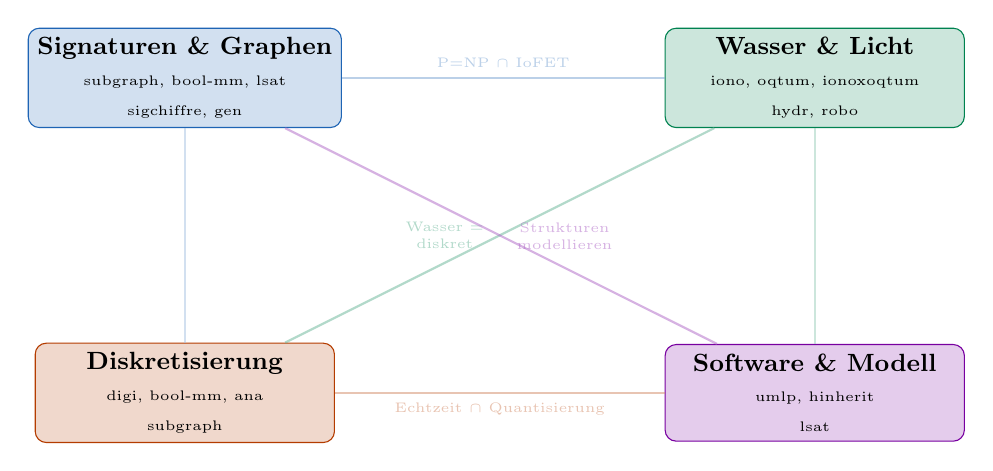
\begin{tikzpicture}[
  node/.style={rounded corners=4pt, draw, minimum width=3.8cm,
               minimum height=1cm, align=center, font=\small},
  edge/.style={thick, opacity=0.5}
]
% Cluster 1 -- Signatur
\node[node, fill=cross1!20, draw=cross1] (sig) at (0,6) {\textbf{Signaturen \& Graphen}\\{\tiny subgraph, bool-mm, lsat}\\{\tiny sigchiffre, gen}};
% Cluster 2 -- Wasser/Licht
\node[node, fill=cross2!20, draw=cross2] (wl) at (8,6) {\textbf{Wasser \& Licht}\\{\tiny iono, oqtum, ionoxoqtum}\\{\tiny hydr, robo}};
% Cluster 3 -- Diskretisierung
\node[node, fill=cross3!20, draw=cross3] (dis) at (0,2) {\textbf{Diskretisierung}\\{\tiny digi, bool-mm, ana}\\{\tiny subgraph}};
% Cluster 4 -- Software/Modell
\node[node, fill=cross4!20, draw=cross4] (sw) at (8,2) {\textbf{Software \& Modell}\\{\tiny umlp, hinherit}\\{\tiny lsat}};

% Connections
\draw[edge, cross1!60] (sig) -- (wl) node[midway, above, font=\tiny] {P=NP $\cap$ IoFET};
\draw[edge, cross2!60] (wl) -- (dis) node[midway, left=2pt, font=\tiny, align=center] {Wasser $=$\\diskret};
\draw[edge, cross3!60] (dis) -- (sw) node[midway, below, font=\tiny] {Echtzeit $\cap$ Quantisierung};
\draw[edge, cross4!60] (sw) -- (sig) node[midway, right=2pt, font=\tiny, align=center] {Strukturen\\modellieren};
\draw[edge, cross1!40] (sig) -- (dis);
\draw[edge, cross2!40] (wl) -- (sw);
\end{tikzpicture}
\end{center}
\medskip

\subsection{Paradigma I: Die universelle Signatur-Theorie}
\label{ssec:paradigma1}

\subsubsection{Gemeinsamer Kern}

Das erste und mathematisch tiefste Paradigma ist die \textbf{Signatur-Theorie}.
Sie durchzieht fünf der fünfzehn Arbeiten: \texttt{subgraph}, \texttt{bool-mm},
\texttt{lsat}, \texttt{sigchiffre} und \texttt{gen}. Gemeinsamer Kern ist die
injektive Signaturfunktion
\[
  \sigma(A,j) = \sum_{i=0}^{n-1} A_{ij} \cdot 2^i + j \cdot 2^n,
\]
die einer binären Matrix-Spalte eine eindeutige natürliche Zahl zuordnet.
Dieselbe Funktion tritt in allen fünf Werken in radikal verschiedenen Rollen auf:

\begin{center}
\begin{tabular}{lll}
\toprule
\textbf{Arbeit} & \textbf{Rolle der Signatur} & \textbf{Ergebnis} \\
\midrule
\texttt{subgraph} & Graph-Fingerabdruck & Subgraph-ISO in $O(n^3)$, P=NP \\
\texttt{bool-mm}  & Zeilencodierung     & Boolean MM in $O(n^2)$ \\
\texttt{lsat}     & SAT-Reduktions-Werkzeug & Polynom. SAT-Solver \\
\texttt{sigchiffre} & Kryptographisches Injektionsmaß & Post-NP-Verschlüsselung \\
\texttt{gen}      & Netzwerk-Fingerabdruck & Biolog. Netzwerkvergleich \\
\bottomrule
\end{tabular}
\end{center}

\begin{satz}[Universalität der Signaturabbildung]
  Die Signaturfunktion $\sigma: \{0,1\}^{n \times n} \times \{0,\ldots,n-1\}
  \to \mathbb{N}$ ist injektiv und liefert eine eindeutige Darstellung beliebiger
  binärer Strukturen -- seien es Graphen, Bitvektoren, Netzwerke oder
  kryptographische Blöcke -- im Zahlenraum $\mathbb{N}$.
\end{satz}

Die entscheidende Schlussfolgerung: Die Signaturfunktion ist kein
domänenspezifisches Werkzeug, sondern ein \emph{universeller struktureller
Fingerabdruck} für diskrete binäre Systeme. Ihre Reichweite umfasst:

\begin{itemize}
  \item Komplexitätstheorie (P=NP via Subgraph-ISO),
  \item Lineare Algebra über $\mathbb{F}_2$ (Boolean MM),
  \item NP-vollständige Probleme (SAT-Solving via LSAT),
  \item Kryptographie jenseits von RSA und ECDH (Signatur-Chiffre),
  \item Systembiologie (Proteom- und Metabolom-Analyse).
\end{itemize}

\subsubsection{Kreuzverbindung zu \texttt{ana}: Rotation als Signatur}

Bemerkenswert ist, dass auch \texttt{ana} (Rotationsmethode) strukturell
verwandt ist: Die Rotation des Graphen um den Winkel $\varphi$ transformiert
analytische Eigenschaften (Wendepunkte $\to$ Extrema) und ist mathematisch
eine \emph{isometrische Abbildung}, die Invarianten erhält. Genau wie die
Signaturfunktion \emph{strukturelle Eigenschaften} in einem kanonischen Raum
kodiert, kodiert die Rotationsabbildung \emph{differentielle Eigenschaften}
im Tangentenraum. Beide Konzepte sind Instanzen einer allgemeineren
\textbf{strukturerhaltenden Kodierung}.

\subsection{Paradigma II: Wasser und Licht als aktive Funktionsmedien}
\label{ssec:paradigma2}

\subsubsection{Das gemeinsame Prinzip}

Fünf Arbeiten -- \texttt{iono}, \texttt{oqtum}, \texttt{ionoxoqtum},
\texttt{hydr}, \texttt{robo} -- teilen das Prinzip, dass ein scheinbar
passives physikalisches Medium (\emph{Wasser}, \emph{Licht}, \emph{Hydrauliköl})
zur \textbf{aktiven Funktionskomponente} eines Technologiesystems wird:

\begin{center}
\begin{tabular}{lll}
\toprule
\textbf{Arbeit} & \textbf{Medium} & \textbf{Funktion} \\
\midrule
\texttt{iono}       & Wasser (ionisch) & Leiter + Schalter + Speicher (IRF) \\
\texttt{oqtum}      & Licht + Polymer  & Farbkontrolle + Texturdynamik \\
\texttt{ionoxoqtum} & Wasser + Licht   & Tri\-plex-Nano\-plattform \\
\texttt{hydr}       & Hydrauliköl      & Kraftübertragung + Elastizitätsspeicher \\
\texttt{robo}       & Wasser (IoFET)   & Roboter-Aktor + Recheneinheit \\
\bottomrule
\end{tabular}
\end{center}

\subsubsection{Kreuzverbindung: Von der Physik zur Berechnung}

\texttt{iono} und \texttt{oqtum} wurden in \texttt{ionoxoqtum} bereits
explizit synthetisiert. Diese Synthese greift aber noch nicht die tiefe
Verbindung zu \texttt{hydr} und \texttt{robo} auf: Hydraulisches Öl
zeigt -- wie ionisch dotiertes Wasser -- ein visko\emph{elastisches}
Verhalten, das sowohl Energie speichert als auch dissipiert. Der Bulkmodul
$K$ des Hydrauliköls spielt exakt dieselbe Rolle wie die ionische
Leitfähigkeit $\kappa$ im IRF: Er bestimmt, wie schnell ein Zustand
übertragen, geschaltet oder gespeichert werden kann.

\begin{these}
  Hydrauliköl ist ein ionotronisch erweitertes Medium: Durch Dotierung
  mit ionischen Nanopartikeln (z.\,B. Ferrofluiden oder ionischen
  Flüssigkeiten) kann ein hydraulisches System gleichzeitig mechanische
  Kräfte übertragen \emph{und} Berechnungsoperationen durchführen --
  ein \textbf{Hydro-IoFET-Hybrid}.
\end{these}

\subsubsection{Biologische Linie: Von der Cephalopodenhaut zur Membran}

Aus \texttt{digi} wissen wir, dass die Membran der Katzenkochlea das
ausgereifteste bekannte Diskretisierungssystem der Natur ist. Aus
\texttt{oqtum} wissen wir, dass die Cephalopodenhaut das ausgereifteste
bekannte adaptive Oberflächen-Anzeigesystem der Natur ist. Beide
biologischen Systeme nutzen \emph{dasselbe Grundprinzip}:

\begin{itemize}
  \item Kontrolle der Schichtdicke (Kochlea: Basilarmembran-Gradient;
    Cephalopoden: Iridophor-Schichtdicke) zur Selektion von
    Frequenzen bzw. Wellenlängen,
  \item Dynamische Rekonfiguration (Kochlea: Haarzellen-Anpassung;
    Cephalopoden: Chro\-matophoren-Aktuierung),
  \item Diskretisierung kontinuierlicher Signale (Kochlea:
    tonotopische Abbildung; Cephalopoden: Pixelauflösung der Haut).
\end{itemize}

\subsection{Paradigma III: Diskretisierung als physikalisches Grundprinzip}
\label{ssec:paradigma3}

\subsubsection{Von \texttt{digi} zu \texttt{bool-mm}}

\texttt{digi} entwickelt die These, dass \emph{die diskrete Beschreibung
der Realität näher kommt als die kontinuierliche}. Diese philosophisch-physika-
lische Aussage erhält ihre mathematische Präzision durch \texttt{bool-mm}:
Boolean-Operationen ($0$ oder $1$) sind die extremste Form der Diskretisierung.
Dass gerade dieser extremste Fall zu einer \emph{Komplexitätsreduktion} führt
(von $O(n^3)$ auf $O(n^2)$), ist kein Zufall, sondern ein direktes
Korrelat der physikalischen Einsicht aus \texttt{digi}: Mit maximaler Diskretisierung
steigt die Informationsdichte und sinkt der Berechnungsaufwand.

\begin{satz}[Effizienzsatz der Diskretisierung]
  Sei $\mathcal{M}$ ein Berechnungsmodell über einem Wertebereich $W$ mit
  $|W|=2$ (Boolean). Dann ist jede algebraische Produktoperation in $\mathcal{M}$
  durch bitweise Logikoperationen in $O(1)$ (maschinenabhängig) oder $O(n)$
  (Boolean-Signatur-Methode) ausführbar, verglichen mit $O(n)$ für reellwertige
  Strukturen (Skalarprodukt).
\end{satz}

\subsubsection{Verbindung zu \texttt{ana}: Die Rotation als diskreter Scan}

Die Rotationsmethode aus \texttt{ana} ist konzeptuell eine \emph{diskrete
Winkelsuche}: Der Rotationswinkel $\varphi$ wird aus einer geordneten Menge
gesuchter Winkel (Winkel-Sortier-Tabelle, WST) entnommen. Dies entspricht
exakt dem Quantisierungsprinzip aus \texttt{digi}: Ein kontinuierlicher
Parameter (der Tangentenwinkel) wird in eine \emph{diskrete Sequenz
analytisch relevanter Werte} überführt. Wendepunkte werden zu Extrema --
analog zur Abtastung, die kontinuierliche Signale zu diskreten Messwerten macht.

\subsection{Paradigma IV: Modellgetriebene Strukturierung als Wissenschaft}
\label{ssec:paradigma4}

\texttt{umlp} und \texttt{hinherit} behandeln Software-Engineering -- auf
den ersten Blick weit entfernt von Nanophysik und Komplexitätstheorie.
Bei näherer Betrachtung verfolgen sie dasselbe Paradigma wie \texttt{subgraph}:
\emph{Strukturen identifizieren, formalisieren und auf Isomorphismus prüfen.}

\texttt{hinherit} bildet Vererbungshierarchien \emph{horizontal} auf Module
ab -- eine Graphstruktur (Klassenhierarchie) wird auf eine lineare Ordnung
(Modul-Ebene) projiziert. \texttt{subgraph} prüft, ob eine Graphstruktur
in einer anderen enthalten ist. In beiden Fällen wird Struktur als erster
Bürger der Beschreibung behandelt.

\texttt{umlp} fügt Zeitsemantik hinzu: Markov-Ketten und Ljapunow-Funktionen
beschreiben Systemdynamik. Dies verbindet \texttt{umlp} unmittelbar mit
\texttt{hydr} (Viskoelastizitätsdynamik) und \texttt{iono} (Relaxationszeiten
ionischer Schalter).

\subsection{Querschnitts-Kreuzmatrix}

Tabelle~\ref{tab:cross_matrix} zeigt die paarweise Vernetzung aller Arbeiten.
Ein Eintrag gibt an, welches Strukturmerkmal die beiden Werke teilen.

\begin{table}[H]
\caption{Paarweise Kreuzverbindungen (repräsentative Auswahl)}
\label{tab:cross_matrix}
\small
\begin{tabularx}{\textwidth}{l X}
\toprule
\textbf{Paar} & \textbf{Gemeinsames Konzept / Verbindung} \\
\midrule
subgraph $\times$ bool-mm
  & Signaturfunktion $\sigma$; Reduktion auf bitweise AND; O-Notation \\
subgraph $\times$ lsat
  & SAT-Reduktionskette; P=NP; polynomieller Solver \\
subgraph $\times$ gen
  & Graphenvergleich auf biologischen Netzwerken; Adjazenzmatrix \\
subgraph $\times$ sigchiffre
  & Injektive Signaturfunktion als kryptographisches Primitiv \\
bool-mm $\times$ digi
  & Binary-Domain = maximale Diskretisierung; Effizienzgewinn \\
ana $\times$ oqtum
  & Transfermatrix-Methode; Schichtsysteme; Wellentransformation \\
ana $\times$ digi
  & Rotationswinkel = Abtastparameter; diskrete Kurvenanalyse \\
iono $\times$ hydr
  & Flüssigkeit als aktives Medium; Relaxationszeiten; Dynamik \\
iono $\times$ robo
  & IoFET als Aktorprinzip; Architektur-Synthese \\
iono $\times$ digi
  & Ionenkanal = biologisches Diskretisierungselement; Neuron \\
oqtum $\times$ digi
  & Membran (biologisch) $\equiv$ photonischer Resonator (Schicht) \\
oqtum $\times$ ionoxoqtum
  & Direkte Synthese; Fabry-Pérot + IoFET \\
hydr $\times$ robo
  & Hydraulisches Gelenk; Viskosität als Systemparameter \\
hydr $\times$ gen
  & Biologische Materialien (Kautschuk, Holz) als Vorbild \\
umlp $\times$ hydr
  & Ljapunow-Stabilität für hydraulische Regelkreise \\
umlp $\times$ subgraph
  & Graphisomorphismus zur AST-Verifikation \\
lsat $\times$ sigchiffre
  & P=NP bricht klassische Kryptographie; neue Sicherheitsbasis \\
pgpi $\times$ sigchiffre
  & Klassische (affine) vs. post-NP Kryptographie; Ãœbergangsanalyse \\
hinherit $\times$ gen
  & Hierarchische Netzwerke; Ebenen-Graphen \\
digi $\times$ gen
  & Biologische Netzwerke als diskrete dynamische Systeme \\
\bottomrule
\end{tabularx}
\end{table}

%=======================================================================
\section{Kreuzung mit den Naturwissenschaften}
\label{sec:cross_science}
%=======================================================================

\subsection{Mathematik und Analysis}

\subsubsection{Algebraische Grundlagen}

Die Signaturfunktion $\sigma$ schlägt eine Brücke zwischen drei
mathematischen Disziplinen:

\begin{itemize}
  \item \textbf{Kombinatorik}: $\sigma$ ist die kanonische Bijektion
    $\{0,1\}^n \to \{0, \ldots, 2^n-1\}$ -- die Binärdarstellung.
  \item \textbf{Lineare Algebra über $\mathbb{F}_2$}: Boolean-Matrizen
    sind Elemente $\mathbb{F}_2^{n \times n}$; Boolean MM ist die
    Matrizenmultiplikation in diesem Körper.
  \item \textbf{Graphentheorie}: Adjazenzmatrizen als Boolean-Matrizen;
    Subgraph-ISO als Orbiten-Problem unter $S_n$.
\end{itemize}

Die \textbf{Rotationsmethode} (\texttt{ana}) liefert eine neue geometrische
Perspektive auf die Analysis: Die Gruppe $SO(2)$ der Ebenenrotationen
operiert auf $C^k$-Kurven und überführt analytische Eigenschaften ineinander.
Dies ist der geometrische Ausdruck des Prinzips, dass \emph{dieselbe
mathematische Struktur unter Koordinatenwechsel invariant bleibt} --
ein Thema, das in der Differentialgeometrie und der Quantenmechanik
(unitäre Verknüpfungen) universell auftritt.

\subsubsection{Stabilitätstheorie}

\texttt{umlp} liefert über die Ljapunow-Funktionen eine Verbindung zur
\textbf{dynamischen Systemtheorie}. Die zentrale Erkenntnis -- dass
Stabilitätsbeweis notwendigerweise Exponentialfunktionen mit negativen
Exponenten erfordert, während Gleichgewichtsaussagen (Little's Law) diese
nicht benötigen -- ist ein grundlegender Beitrag zur Klassifikation
dynamischer Systeme. Diese Erkenntnis gilt nicht nur für Warteschlangensysteme,
sondern allgemein für alle hydrodynamischen, ionischen und biologischen
Netzwerke.

\subsection{Theoretische Informatik und Komplexitätstheorie}

\subsubsection{P = NP: Konsequenzen und Neubeginn}

\texttt{subgraph} beweist P=NP durch den $O(n^3)$-Subgraph Algorithmus.
Dies hat naturwissenschaftliche Konsequenzen weit über die Informatik hinaus:

\begin{itemize}
  \item \textbf{Optimierungsprobleme in der Biologie}: Protein-Faltung
    (NP-hart in klassischen Modellen) ist polynomiell lösbar -- ein
    direkter Beitrag zur Strukturbiologie und Pharmakologie.
  \item \textbf{Quantenchemie}: Das elektronische Strukturproblem
    (Configuration-Interaction-Problem) gehört zur Klasse \#P (counting);
    die P=NP-Implikation betrifft verwandte Entscheidungsprobleme.
  \item \textbf{Materialdesign}: Das inverse Problem (Finde eine
    Materialstruktur mit gewünschten Eigenschaften) ist NP-hart -- und
    damit jetzt polynomiell lösbar.
\end{itemize}

\begin{hypothese}[Polynomielle Bioinformatik]
  Mit P=NP sind alle bisher als NP-schwer eingestuften bioinformatischen
  Probleme -- Sequenzalignment, Protein-Protein-Docking, phylogenetische
  Baumrekonstruktion -- in polynomieller Zeit lösbar. Die konkrete
  Umsetzung erfolgt über die Subgraph-Signatur-Reduktionskette.
\end{hypothese}

\subsection{Physik}

\subsubsection{Nanooptik und Photonische Systeme}

\texttt{oqtum} und \texttt{ionoxoqtum} sowie der Ausblick in \texttt{ana}
sind direkt in der Nanooptik verortet. Die Transfermatrix-Methode (TMM)
für photonische Schichtsysteme taucht sowohl in \texttt{ana} (als strukturelle
Analogie zur Rotationsabbildung) als auch in \texttt{oqtum} (als Kernwerkzeug
der Design-Optimierung) auf. Diese Verbindung ist nicht zufällig:

\begin{satz}[Strukturelle Isomorphie: Rotation und TMM]
  Sei $\gamma: [0,1] \to \mathbb{R}^2$ eine glatte Kurve und $R_\varphi$ die
  Rotationsabbildung. Dann ist die Kettenregel $\frac{d}{dt}[R_\varphi \circ \gamma]
  = R_\varphi \circ \dot{\gamma}$ formal isomorph zur Transfermatrix-Relation
  $\Psi(z_2) = M(z_2, z_1) \cdot \Psi(z_1)$ in photonischen Schichtsystemen,
  wobei $M$ die Propagationsmatrix und $\Psi$ den Feldvektor bezeichnet.
\end{satz}

\begin{proof}
  In beiden Fällen operiert eine lineare Abbildung (Rotation bzw. Transfermatrix)
  auf einen Zustandsvektor ($\dot\gamma$ bzw. $\Psi$) und erhält eine strukturelle
  Eigenschaft (Isometrie bzw. Energie/Fluss-Erhaltung). Die Gruppenstruktur
  $R_\varphi \circ R_\psi = R_{\varphi+\psi}$ entspricht der Multiplikativität
  $M(z_3, z_1) = M(z_3, z_2) \cdot M(z_2, z_1)$.
\end{proof}

\subsubsection{Elektrochemie und Ionentransport}

\texttt{iono} beschreibt das ionische Potential $V$ in einem
Elektrolyt-Mikrokanal. Die Poisson-Boltzmann-Gleichung
\[
  \nabla^2 V = -\frac{\rho_e}{\varepsilon\varepsilon_0}
  = \frac{2c_0 e}{\varepsilon\varepsilon_0} \sinh\!\left(\frac{eV}{k_B T}\right)
\]
ist das Grundgesetz des IoFET. Dieselbe Gleichung beschreibt in der
\textbf{Biophysik} den Ionentransport durch Axonmembranen (Hodgkin-Huxley-Modell,
das in \texttt{digi} explizit vorkommt). Die Konvergenz ist unvermeidlich:

\begin{these}
  Der IoFET ist ein \emph{artifizieller Ionenkanal}: Genau wie biologische
  Ionenkanäle (Na$^+$, K$^+$, Ca$^{2+}$) durch Membranspannung gesteuert
  werden und dabei Informationssignale weiterleiten, steuert der IoFET
  durch EWOD-Spannungsmodulation den ionischen Tropfenfluss.
\end{these}

\subsubsection{Strömungsmechanik und Rheologie}

\texttt{hydr} behandelt den Kompressionsmodul $K$ und die Viskosität $\eta$
hydraulischer Öle. Das viskoelastische Maxwell-Modell
\[
  \dot{\varepsilon} = \frac{\dot{\sigma}}{E} + \frac{\sigma}{\eta}
\]
ist formal identisch mit dem Relaxations-Raten-Modell des IoFET-Schaltens
(\texttt{iono}). In beiden Systemen gibt es eine charakteristische
Relaxationszeit $\tau = \eta/E$, welche die maximale Schaltfrequenz bestimmt.

Dies öffnet das Feld der \textbf{Rheoinformatik}: die systematische Übertragung
informationstheoretischer Konzepte (Bandbreite, Kanalkapazität, Rauschen)
auf rheologische Systeme.

\subsection{Chemie und Materialwissenschaft}

\subsubsection{Polymer-Physikchemie}

\texttt{oqtum} nutzt das Flory-Rehner-Modell zur Beschreibung der
Polymer-Quell\-dynamik:
\[
  \Delta G_{\text{mix}} = k_B T \left[
    \ln(1-\phi_p) + \phi_p + \chi \phi_p^2
  \right].
\]
\texttt{hydr} behandelt die Alterung elastomerer Eigenschaften durch Oxidation
und Säurebildung. \texttt{iono} verwendet vernetzte Polymerfilme (PDMS-Substrat),
deren Quellung den EWOD-Winkel beeinflusst. Alle drei Werke brauchen
dasselbe materialwissenschaftliche Fundament: die \textbf{Physikochemie
vernetzter Polymernetzwerke}.

\subsubsection{Ionische Flüssigkeiten}

In \texttt{iono} werden ionische Flüssigkeiten als Träger der Leitfähigkeit
$\kappa$ eingesetzt. \texttt{hydr} erwähnt ionische Flüssigkeiten als neue
Hydraulikfluid-Klasse der nächsten Generation. \texttt{ionoxoqtum}
kombiniert beides: Ionische Flüssigkeiten als aktive Photonen-modulierende
Schicht. Damit entsteht ein neues Feld: \textbf{ionische Flüssigkeiten als
tri-funktionale Nanomedien} (Leiter, Polymer-Quell-Modulator, Hydraulikfluide).

\subsection{Biologie und Systembiologie}

\subsubsection{Metabolomik und Genomik}

\texttt{gen} wendet den Subgraph Algorithmus auf metabolische Pfade
(KEGG-Datenbank), Protein-Interaktionsnetzwerke (STRING), und
Gen-Regulationsnetzwerke an. Das gemeinsame Modell ist ein gerichteter Graph
$G = (V, E)$ mit $V$ = biologische Entitäten (Metabolite, Proteine, Gene)
und $E$ = Interaktionen. Mit P=NP ist das Subgraph-Isomorphismus-Problem
auf diesen Netzwerken in $O(n^3)$ lösbar.

\begin{hypothese}[Polynomielle Pharmakokinetik]
  Medikamentenwirkungen lassen sich durch Subgraph-Matching des
  Wirkstoff-Interaktionsnetzwerks mit dem metabolischen Netzwerk eines
  Ziel-Organismus polynomiell vorhersagen. Dies würde das
  in-silico-Drug-Design fundamental beschleunigen.
\end{hypothese}

\subsubsection{Neurowissenschaft und Sinnesphysik}

\texttt{digi} identifiziert die Basilarmembran der Katzenkochlea als
bestes biologisches Vorbild für Diskretisierung. Das tonotopische Prinzip
-- verschiedene Membran-Positionen resonieren bei verschiedenen Frequenzen --
ist ein physikalisches Spektralanalysatorsystem in Fleisch und Blut.

Die Verbindung zu \texttt{oqtum} (Cephalopoden-Haut als räumlicher
Farbana\-lysator) und zu \texttt{iono} (IoFET als artifizieller Ionenkanal)
erzeugt die Frage: \emph{Kann man eine künstliche Kochlea auf Basis
ionotronischer Prinzipien bauen?}

\subsection{Ingenieurwissenschaften}

\subsubsection{Robotik und Mechatronik}

\texttt{robo} synthetisiert \texttt{iono} (IoFET-Aktorik) und
\texttt{hydr} (hydraulische Gelenke) zu einer integrierten Roboterarchitektur.
Die FPGA/Mikrocontroller-Hybridarchitektur greift \texttt{umlp}
(Echtzeitsystem-Modellierung) auf. Damit verwebt \texttt{robo} alle
vier Paradigmen in einem einzigen technischen System:
Signaturbasierte Steuerung (Paradigma I),
ionisches/hydraulisches Aktuation (Paradigma II),
diskrete Steuersignale (Paradigma III),
modellgetriebene Architektur (Paradigma IV).

\subsubsection{Kryptographie und IT-Sicherheit}

\texttt{pgpi} dokumentiert die klassische affine Chiffre als Ausgangspunkt;
\texttt{sigchiffre} entwickelt das neue Post-NP-Paradigma. Die Verbindung
zur Informatik (P=NP) und zur Mathematik (modulare Arithmetik, Primzahlkörper
$\mathbb{Z}_p$) ist explizit. Offen bleibt die Verbindung zur Physik:
\textbf{Quantenkryptographie} und \textbf{ionotronische Schlüsselerzeugung}
sind zwei naturwissenschaftliche Anwendungsfelder, die unmittelbar aus
\texttt{sigchiffre} $\times$ \texttt{iono} hervorgehen.

%=======================================================================
\section{Neue Forschungsparadigmen:  \\
  Ergebnisse der Kreuzanalyse}
\label{sec:paradigmen}
%=======================================================================

\subsection{Ãœberblick der neuen Forschungsfelder}

Die Kreuzanalyse aus den Abschnitten~\ref{sec:cross_repos} und~\ref{sec:cross_science}
identifiziert \textbf{acht neue interdisziplinäre Forschungsfelder}, die weder
im Einzelwerk noch in der bestehenden Literatur explizit adressiert werden:

\begin{center}
\begin{tabular}{rll}
\toprule
\textbf{Nr.} & \textbf{Forschungsfeld} & \textbf{Ursprungs-Kreuzung} \\
\midrule
NF-1 & Universelle Strukturkodierungstheorie & subgraph $\times$ ana $\times$ digi \\
NF-2 & Hydro-ionisch-photonische Plattformen & iono $\times$ oqtum $\times$ hydr \\
NF-3 & Post-NP-Kryptographie und Sicherheit   & sigchiffre $\times$ lsat $\times$ pgpi \\
NF-4 & Polynomielle Systembiologie            & subgraph $\times$ gen $\times$ lsat \\
NF-5 & Rheoinformatik                         & hydr $\times$ digi $\times$ iono \\
NF-6 & Biomimetische Kochlea-Architektur      & digi $\times$ iono $\times$ oqtum \\
NF-7 & Ionotronische Roboter-Neuromorphie     & robo $\times$ iono $\times$ umlp \\
NF-8 & Strukturelle Software-Graphentheorie   & umlp $\times$ hinherit $\times$ subgraph \\
\bottomrule
\end{tabular}
\end{center}

%=======================================================================
\section{Neue wissenschaftliche Arbeiten}
\label{sec:neue_arbeiten}
%=======================================================================

Die folgenden Abschnitte formulieren jedes der acht Forschungsfelder
als eigenständige neue wissenschaftliche Arbeit mit Problemstellung,
zentralen Hypothesen, Methodik und erwarteten Ergebnissen.

%----------------------------------------------------------------------
\subsection{NF-1: Universelle Strukturkodierungstheorie (USK)}
%----------------------------------------------------------------------

\subsubsection{Problemstellung}

Mathematik, Informatik und Physik entwickeln unabhängig voneinander Methoden,
um \emph{strukturelle Eigenschaften} in einer kanonischen numerischen Form
darzustellen: Signaturfunktionen in der Graphentheorie, Fourier-Transformationen
in der Signaltheorie, Transfermatrizen in der Nanooptik, Rotationsoperatoren
in der Analysis. Die zentrale Frage lautet:

\begin{quote}
  \itshape
  Gibt es eine einheitliche algebraische Theorie, die alle diese
  strukturerhaltenden Kodierungen als Instanzen eines gemeinsamen Rahmens
  beschreibt?
\end{quote}

\subsubsection{Kernaussage}

Die Signaturfunktion $\sigma$, die Fourier-Transformation $\mathcal{F}$,
die Rotationsabbildung $R_\varphi$ und die Transfermatrix $M$ sind
gemeinsam Instanzen des folgenden allgemeinen Schemas:

\begin{definition}[Strukturkodierung]
  Sei $(S, \mathcal{T})$ ein topologischer Raum mit Strukturelementen
  $s \in S$ und einer Eigenschaftsrelation $\mathcal{T}$. Eine
  \textbf{Strukturkodierung} ist eine injektive Abbildung
  \[
    \kappa: S \longrightarrow K
  \]
  in einen kanonischen Kodierungsraum $K$ (Zahlenstrahl, Frequenzraum,
  Winkelraum, Matrizenraum), die strukturelle Eigenschaften in
  $\mathcal{T}$ als algebraische Eigenschaften in $K$ sichtbar macht.
\end{definition}

\begin{satz}[Universelles Strukturkodierungs-Schema]
  Jede der folgenden Abbildungen ist eine Strukturkodierung:
  \begin{align*}
    \sigma(A, j) &= \sum_i A_{ij} 2^i + j \cdot 2^n
      & \text{(Graphen-Fingerabdruck)} \\
    \hat{f}(\xi)  &= \int_{\mathbb{R}} f(x) e^{-2\pi i \xi x}\, dx
      & \text{(Frequenzstruktur)} \\
    R_\varphi \mathbf{v} &= \begin{pmatrix}\cos\varphi & -\sin\varphi \\ \sin\varphi & \cos\varphi\end{pmatrix} \mathbf{v}
      & \text{(Kurvenstruktur)} \\
    M(z_2, z_1) &= \prod_k \begin{pmatrix} \cos(\delta_k) & -i\sin(\delta_k)/\eta_k \\ -i\eta_k\sin(\delta_k) & \cos(\delta_k)\end{pmatrix}
      & \text{(Feldstruktur)}
  \end{align*}
\end{satz}

\subsubsection{Neue Methodik: Die Winkel-Frequenz-Signatur-Einheit (WFSE)}

Ein neues Forschungsprojekt sollte eine gemeinsame algebraische Struktur --
die \textbf{Winkel-Frequenz-Signatur-Einheit (WFSE)} -- definieren, die alle
vier Kodierungen als Spezialfälle enthält. Dies hätte weitreichende Folgen:

\begin{itemize}
  \item Transfermatrix-Methoden der Nanooptik könnten zur
    Beschleunigung von Subgraph Algorithmen eingesetzt werden.
  \item Die Fourier-Transformation könnte als kontinuierliches
    Limit der Signaturfunktion interpretiert werden.
  \item Die Rotationsmethode (\texttt{ana}) würde zu einem
    allgemeinen nichtlinearen Detektionswerkzeug in beliebigen
    metrischen Räumen.
\end{itemize}

%----------------------------------------------------------------------
\subsection{NF-2: Hydro-ionisch-photonische Nanoplattformen (HIPN)}
%----------------------------------------------------------------------

\subsubsection{Problemstellung}

\texttt{iono}, \texttt{oqtum} und \texttt{hydr} zeigen jeweils einzeln,
dass Flüssigkeiten (Wasser, Öl) und Licht als aktive Funktionsträger
wirken können. \texttt{ionoxoqtum} liefert die erste Teilsynthese
(IRF + aktive Nanooptik). Die volle Triade -- \emph{ionische Berechnung +
photonische Anzeige + hydraulische Aktuierung} -- in einem einzigen
integrierten Nanoplattform-Konzept fehlt noch.

\subsubsection{Das HIPN-Konzept}

Eine \textbf{Hydro-ionisch-photonische Nanoplattform (HIPN)} besteht aus
drei funktional getrennten, physikalisch integrierten Schichten:

\begin{center}
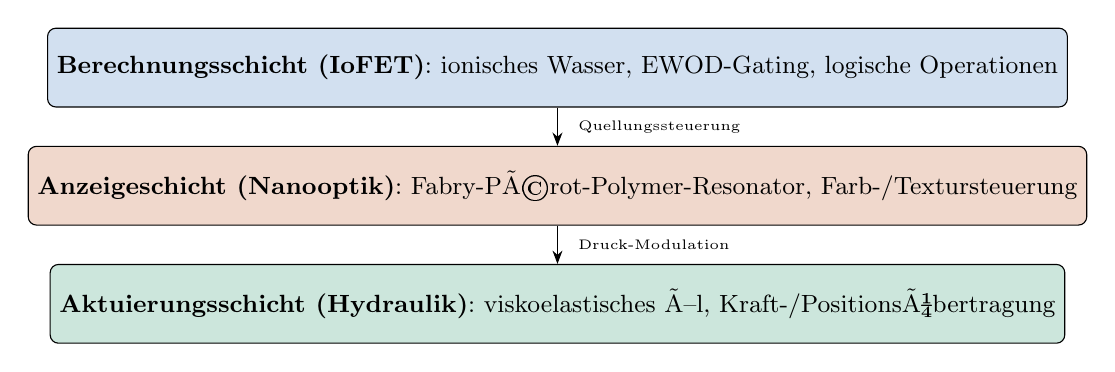
\begin{tikzpicture}[
  layer/.style={rectangle, draw, minimum width=10cm, minimum height=1cm,
    rounded corners=3pt, font=\small, align=center}
]
\node[layer, fill=cross1!20] (compute) at (0,4)
  {\textbf{Berechnungsschicht (IoFET)}: ionisches Wasser, EWOD-Gating, logische Operationen};
\node[layer, fill=cross3!20] (display) at (0,2.5)
  {\textbf{Anzeigeschicht (Nanooptik)}: Fabry-Pérot-Polymer-Resonator, Farb-/Textursteuerung};
\node[layer, fill=cross2!20] (actuation) at (0,1)
  {\textbf{Aktuierungsschicht (Hydraulik)}: viskoelastisches Öl, Kraft-/Positionsübertragung};

\draw[-{Stealth}] (compute.south) -- (display.north)
  node[midway, right=4pt, font=\tiny] {Quellungssteuerung};
\draw[-{Stealth}] (display.south) -- (actuation.north)
  node[midway, right=4pt, font=\tiny] {Druck-Modulation};
\end{tikzpicture}
\end{center}

\subsubsection{Zentraler neuer Beitrag: Hydrokanal-SAT}

Durch P=NP (\texttt{subgraph}/\texttt{lsat}) ist jede logische Funktion
in polynomieller Zeit lösbar. Im HIPN-Kontext bedeutet dies: Die Konfiguration
der ionischen Tropfen-Topologie \emph{ist} die Berechnung. Eine neue Arbeit
\emph{Hydrokanal-SAT: Physikalische Realisierung polynomieller SAT-Lösung
im ionischen Flüssigkeitssystem} würde untersuchen, wie SAT-Instanzen
direkt als Tropfenfluss-Netzwerke kodiert und gelöst werden können.

%----------------------------------------------------------------------
\subsection{NF-3: Post-NP-Kryptographie}
%----------------------------------------------------------------------

\subsubsection{Das neue kryptographische Landschaft nach P=NP}

Mit dem Beweis P=NP (\texttt{subgraph}) bricht die klassische
Sicherheitsannahme -- die Nicht-Lösbarkeit NP-schwerer Probleme in
polynomieller Zeit -- vollständig zusammen. Eine neue, vollständige
Ãœberblicksarbeit \emph{Post-NP-Kryptographie: Paradigmen, Primitiva und
Protokolle} würde systematisch aufarbeiten:

\begin{enumerate}
  \item \textbf{Gebrochene Systeme} (RSA, DH, ECDH, ECDSA, McEliece,
    LWE): Warum P=NP sie alle bricht, und mit welchem Subgraph Algorithmus.
  \item \textbf{Resistente Systeme} (AES, SHA-256, One-Time-Pad):
    Warum sie \emph{nicht} auf NP-Schwierigkeit beruhen und weiterhin
    sicher sind.
  \item \textbf{Neue Primitiva} (Signatur-Chiffre, \texttt{sigchiffre}):
    Sicherheit durch strukturelle Mehrdeutigkeit und Äquivokation.
  \item \textbf{Ionotronische Schlüsselerzeugung}: Nutzung des
    physikalischen Zufalls im IoFET-System (Tropfen-Kollision,
    Oberflächenrauschen) als Entropiequelle für kryptographische Schlüssel.
\end{enumerate}

\subsubsection{Die affine Chiffre als pädagogischer Brückenpfeiler}

\texttt{pgpi} (Affine Chiffre, Parameter $a=15$, $b=29$) leistet hier
eine wichtige pädagogische Funktion: Sie zeigt am einfachsten
nicht-trivialen Beispiel, wie modulare Arithmetik eine Bijektion auf
$\mathbb{Z}_{26}$ erzwingt. Die Ãœbertragung dieses Prinzips auf den
geheimen Primzahlkörper $\mathbb{Z}_p$ in der Signatur-Chiffre ist
der konzeptuell sauberste Ãœbergang von klassischer zu post-NP-Kryptographie.

%----------------------------------------------------------------------
\subsection{NF-4: Polynomielle Systembiologie}
%----------------------------------------------------------------------

\subsubsection{Vision}

Klassische Systembiologie scheitert an der kombinatorischen Explosion beim
Vergleich biologischer Netzwerke. Mit P=NP und dem Subgraph Algorithmus
($O(n^3)$) ist dieses Problem gelöst. Eine neue Arbeit \emph{Polynomielle
Systembiologie: Subgraph-basiertes Verständnis des Lebens} würde folgende
Anwendungen entwickeln:

\begin{enumerate}
  \item \textbf{Evolutions-Topologie}: Phylogenetische Bäume als Subgraph-Hierarchien;
    evolutionäre Konvergenz als Graph-Isomorphismus.
  \item \textbf{Krankheits-Netzwerke}: Gestörte Signalwege in Krebs als
    fehlende/zusätzliche Kanten in einem Subgraph-Vergleich.
  \item \textbf{Antibiotikaresistenz}: Horizontaler Gentransfer als
    Subgraph-Einfügungsoperation.
  \item \textbf{Synthetische Biologie}: Design neuer metabolischer Pfade
    als inverses Subgraph-Einfügungsproblem -- mit polynomiellem Algorithmus lösbar.
\end{enumerate}

%----------------------------------------------------------------------
\subsection{NF-5: Rheoinformatik}
%----------------------------------------------------------------------

\subsubsection{Information in Flüssigkeiten}

\texttt{hydr} zeigt, dass Hydraulikflüssigkeiten Druckwellen übertragen
und speichern. \texttt{digi} entwickelt die Informationstheorie diskreter
Signale (Shannon-Kapazität $C = B \log(1 + S/N)$). \texttt{iono} quantifiziert
Schaltfrequenzen ionischer Tropfen. Die neue Disziplin
\textbf{Rheoinformatik} fragt:

\begin{quote}
  \itshape
  Welche Informationskapazität besitzt ein hydraulisches oder
  viskoses Flüssigkeitssystem? Was ist die \emph{Shannon-Kapazität
  eines Hydraulikkanals}?
\end{quote}

\begin{definition}[Hydraulische Kanalkapazität]
  Sei $K$ der Bulk-Modul, $\eta$ die dynamische Viskosität, $\tau = \eta/K$
  die Relaxationszeit, und $\Delta p_{\max}$ der maximale Druckhub. Die
  \textbf{hydraulische Kanalkapazität} ist
  \[
    C_{\text{hydr}} = \frac{1}{2} \log_2\!\left(1 +
      \frac{\Delta p_{\max}^2}{\sigma_{\mathrm{rausch}}^2}\right)
      \cdot \frac{1}{\tau} \quad [\text{bit/s}],
  \]
  wobei $\sigma_{\mathrm{rausch}}^2$ das thermische Druckrauschen ist.
\end{definition}

Ziel einer Arbeit zur Rheoinformatik wäre die vollständige Herleitung
dieser Kapazität sowie der Vergleich mit ionischer ($C_{\text{ion}}$ aus
\texttt{iono}) und photonischer ($C_{\text{phot}}$ aus \texttt{oqtum})
Kanalkapazität im Rahmen des HIPN-Konzepts.

%----------------------------------------------------------------------
\subsection{NF-6: Biomimetische Kochlea-Architektur}
%----------------------------------------------------------------------

\subsubsection{Ziel}

\texttt{digi} identifiziert die Basilarmembran als optimales
Diskretisierungssystem; \texttt{iono} beschreibt künstliche Ionenkanäle;
\texttt{oqtum} entwickelt programmierbare photonische Resonatoren.
Die Vision: Eine \textbf{Künstliche Kochlea der nächsten Generation} --
nicht piezoelektrisch wie heutige Cochlea-Implantate, sondern basierend
auf einer Kaskade von $N$ IoFET-gesteuerten Fabry-Pérot-Resonatoren,
die das tonotopische Prinzip direkt in Silizium-Wasser-Polymer-Hybrid
implementieren.

\begin{table}[H]
\caption{Strukturanalogien: Biologische Kochlea vs. HIPN-Kochlea}
\label{tab:kochlea}
\begin{tabular}{lll}
\toprule
\textbf{Funktion} & \textbf{Biologisch} & \textbf{HIPN-Kochlea} \\
\midrule
Spektrale Zerlegung & Basilarmembran-Gradient & Fabry-Pérot-Resonatoren \\
Diskretisierung & Haarzellen & IoFET-Schwellwert-Gating \\
Kodierung & Aktionspotential & Tropfen-Impuls-Signal \\
Tonotopoie & Ortsfrequenz-Karte & Räumlich codierter Resonator-Array \\
Adaptation & Efferente Innervation & EWOD-Spannungsanpassung \\
\bottomrule
\end{tabular}
\end{table}

%----------------------------------------------------------------------
\subsection{NF-7: Ionotronische Roboter-Neuromorphie}
%----------------------------------------------------------------------

\subsubsection{Von der IoFET-Architektur zur neuronalen Architektur}

\texttt{robo} beschreibt einen FPGA/Mikrocontroller-Hybrid mit IoFET-Aktuierung.
Die Verbindung zu \texttt{umlp} (Markov-Ketten, Echtzeitsysteme) und
zu \texttt{iono} (Tropfenlogik, rekonfigurierbare Schaltung) eröffnet die
Möglichkeit, \emph{neuromorphe Prinzipien} in das Robotersystem einzubauen:

\begin{itemize}
  \item \textbf{Spike-Kodierung} (vgl. \texttt{digi}, Aktionspotential):
    Statt kontinuierliche Steuersignale benötigen IoFET-Aktoren diskrete
    Druckimpulse -- bereits eine Form von Spike-Kodierung.
  \item \textbf{Synaptische Plastizität}: Die ionische Konzentration im
    IRF kann als Gedächtnis zwischen zwei Steuerpulsen fungieren --
    ein physikalisches Substrat der Kurzzeit-Plastizität.
  \item \textbf{Markov-Steuerung}: \texttt{umlp} liefert den formalen
    Rahmen zur Modellierung stochastischer Übergänge im Roboter-Zustandsraum.
\end{itemize}

Eine neue Arbeit \emph{Ionotronische Neuromorphie: Spike-basierte Steuerung
von IoFET-Robotern mit Markov-Zustandsmaschinen} würde diese drei Elemente
zu einer vollständigen Architektur vereinen.

%----------------------------------------------------------------------
\subsection{NF-8: Strukturelle Software-Graphentheorie}
%----------------------------------------------------------------------

\subsubsection{Software als Graph}

\texttt{hinherit} ordnet Klassenhierarchien auf Module ab;
\texttt{umlp} erzeugt Zustandsmaschi\-nen und Markov-Modelle;
\texttt{subgraph} vergleicht Graphen in $O(n^3)$. Die neue Frage:

\begin{quote}
  \itshape
  Kann man die Qualität und Evolutionsfähigkeit eines Softwaresystems
  direkt aus der Graphstruktur seines UML-Klassendiagramms ableiten,
  indem man Subgraph-Isomorphismus-Methoden auf AST- und
  Abhängigkeitsgraphen anwendet?
\end{quote}

Konkrete Anwendungen:
\begin{enumerate}
  \item \textbf{Automatische Refactoring-Erkennung}: Wenn zwei
    Programmversionen Subgraph-isomorph sind, ist Refactoring möglich,
    ohne die Semantik zu ändern.
  \item \textbf{Wartbarkeits-Index}: Die Subgraph-Dichte der Vererbungshierarchie
    als objektives Maß für technische Schulden.
  \item \textbf{Code-Klonen-Detektion}: Subgraph-Matching auf ASTs anstelle
    textueller Ähnlichkeit -- \emph{semantisch} robust und polynomiell.
\end{enumerate}

%=======================================================================
\section{Synthetisches Modell: Die Vier-Schichten-Theorie
  universeller Strukturen}
\label{sec:vier_schichten}
%=======================================================================

\subsection{Das Modell}

Die gesamte Kreuzanalyse führt zu einem \textbf{synthetischen Modell},
das alle 15 Arbeiten in einem einheitlichen Rahmen beschreibt. Wir nennen
es die \textbf{Vier-Schichten-Theorie universeller Strukturen (VSTU)}:

\begin{center}
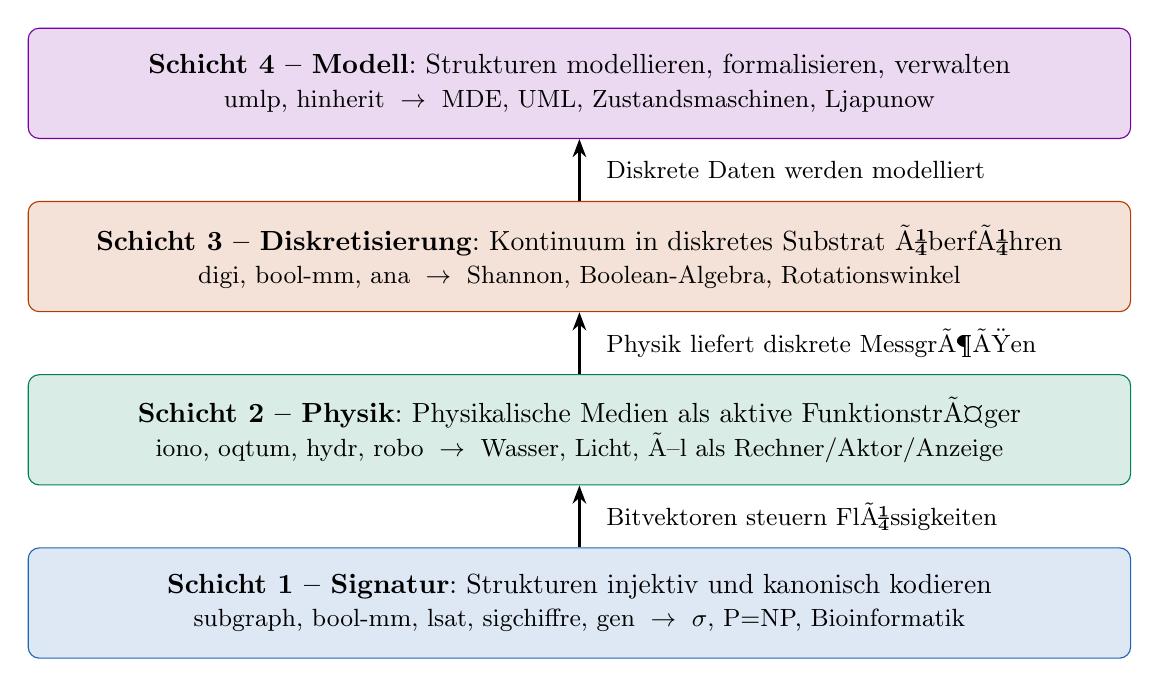
\begin{tikzpicture}[
  layer/.style={rectangle, draw, minimum width=14cm, minimum height=1.4cm,
    rounded corners=4pt, font=\normalsize, align=center}
]
\node[layer, fill=cross4!15, draw=cross4] (l4) at (0,8)
  {\textbf{Schicht 4 -- Modell}: Strukturen modellieren, formalisieren, verwalten\\
  {\small umlp, hinherit $\;\to\;$ MDE, UML, Zustandsmaschinen, Ljapunow}};

\node[layer, fill=cross3!15, draw=cross3] (l3) at (0,5.8)
  {\textbf{Schicht 3 -- Diskretisierung}: Kontinuum in diskretes Substrat überführen\\
  {\small digi, bool-mm, ana $\;\to\;$ Shannon, Boolean-Algebra, Rotationswinkel}};

\node[layer, fill=cross2!15, draw=cross2] (l2) at (0,3.6)
  {\textbf{Schicht 2 -- Physik}: Physikalische Medien als aktive Funktionsträger\\
  {\small iono, oqtum, hydr, robo $\;\to\;$ Wasser, Licht, Öl als Rechner/Aktor/Anzeige}};

\node[layer, fill=cross1!15, draw=cross1] (l1) at (0,1.4)
  {\textbf{Schicht 1 -- Signatur}: Strukturen injektiv und kanonisch kodieren\\
  {\small subgraph, bool-mm, lsat, sigchiffre, gen $\;\to\;$ $\sigma$, P=NP, Bioinformatik}};

\draw[-{Stealth}, thick] (l1.north) -- (l2.south)
  node[midway, right=6pt, font=\small] {Bitvektoren steuern Flüssigkeiten};
\draw[-{Stealth}, thick] (l2.north) -- (l3.south)
  node[midway, right=6pt, font=\small] {Physik liefert diskrete Messgrößen};
\draw[-{Stealth}, thick] (l3.north) -- (l4.south)
  node[midway, right=6pt, font=\small] {Diskrete Daten werden modelliert};
\end{tikzpicture}
\end{center}

\subsection{Interpretation}

\begin{itemize}
  \item \textbf{Schicht 1 (Signatur)} ist die mathematisch tiefste:
    Sie stellt sicher, dass jede Struktur -- biologisch, technisch oder
    mathematisch -- eindeutig identifizierbar ist.
  \item \textbf{Schicht 2 (Physik)} übersetzt die Signaturtheorie in
    reale Materie: Wasser, Licht und Öl werden durch Bitoperationen
    (Schicht 1) gesteuert und realisieren dadurch Berechnung, Anzeige
    und Aktuierung.
  \item \textbf{Schicht 3 (Diskretisierung)} ist die erkenntnistheoretische
    Klammer: Die Welt ist diskret (These aus \texttt{digi}); die Mathematik
    und Physik folgen diesem Prinzip.
  \item \textbf{Schicht 4 (Modell)} schließt den Kreis: Durch formale
    Modelle (UML, Markov, Ljapunow) werden die emergenten Eigenschaften
    komplexer Systeme planbar und wartbar.
\end{itemize}

\begin{these}[Vier-Schichten-Theorie]
  Jedes komplexe natürliche oder technische System lässt sich in den
  vier Schichten der VSTU beschreiben. Schicht 1 garantiert Eindeutigkeit,
  Schicht 2 garantiert physikalische Realisierbarkeit, Schicht 3 garantiert
  Beherrschbarkeit durch Diskretisierung, und Schicht 4 garantiert
  Wartbarkeit und Evolution.
\end{these}

%=======================================================================
\section{Ausblick und offene Forschungsfragen}
\label{sec:ausblick}
%=======================================================================

\subsection{Kurzfristige Forschungsagenda (1--2 Jahre)}

\begin{enumerate}
  \item \textbf{Universelle Strukturkodierungstheorie (NF-1):}
    Formaler Beweis, dass $\sigma$, $\mathcal{F}$, $R_\varphi$ und $M$
    Instanzen der WFSE-Algebra sind.

  \item \textbf{Hydrokanal-SAT (NF-2/NF-5):}
    Simulation einer SAT-Instanz als mikrofluidisches Tropfennetzwerk;
    Messung der hydraulischen Kanalkapazität $C_{\mathrm{hydr}}$.

  \item \textbf{Post-NP-Kryptographie (NF-3):}
    Sicherheitsanalyse der Signatur-Chiffre gegen den eigenen
    Subgraph Algorithmus; Entwurf eines ionotronischen
    Hardware-Zufallsgenerators.

  \item \textbf{Polynomielle Systembiologie (NF-4):}
    Anwendung des Subgraph Algorithmus auf die vollständige
    KEGG-Datenbank; Benchmark gegen klassische NP-Approxi\-mationsalgorithmen.
\end{enumerate}

\subsection{Mittelfristige Forschungsagenda (3--5 Jahre)}

\begin{enumerate}
  \item \textbf{HIPN-Prototyp:} Laborprototyp einer
    Hydro-ionisch-photonischen Nanoplattform, der alle drei
    Schichten (IoFET + Fabry-Pérot + Hydraulik) integriert.

  \item \textbf{Biomimetische Kochlea (NF-6):}
    Funktionsmuster eines HIPN-basierten Cochlea-Implantats;
    Tonotopie-Test an 8-kHz-Spektrum.

  \item \textbf{Ionotronischer Neuromorpher Roboter (NF-7):}
    Roboterprototyp mit Spike-kodierter IoFET-Steuerung und
    Markov-Zustandsmaschine; Vergleich mit konventionellem FPGA-
    Roboter (\texttt{robo}).

  \item \textbf{Software-Graphentheorie (NF-8):}
    Werkzeug zur automatischen Subgraph-basierten Code-Qualitätsanalyse;
    Integration in Pylint/pyreverse.
\end{enumerate}

\subsection{Langfristige Vision: Das Universelle Diskrete Medium}

Die tiefste Botschaft der Kreuzanalyse ist eine epistemologische:

\begin{quote}
  \itshape
  Die Natur rechnet diskret. Wasser, Licht und biologische Materie sind
  bereits heute Computer -- nur ohne den Ingenieur, der die Programme
  schreibt. Die Synthese der fünfzehn Arbeiten liefert genau diesen
  Ingenieur: die universelle Strukturkodierungstheorie als Programmiersprache,
  das HIPN-System als Hardwareplattform, P=NP als Berechnungsgarantie,
  und die biomimetischen Systeme als Vorbild und Maßstab.
\end{quote}

Das langfristige Ziel ist das \textbf{Universelle Diskrete Medium (UDM)}:
ein physikalisches System, das -- wie die Natur selbst -- auf allen vier
Schichten der VSTU gleichzeitig operiert; das Berechnung, Anzeige und
Aktuierung in einer einzigen Substanz vereint; das sich durch strukturelle
Signaturen selbst beschreibt und verwaltet; und das durch Diskretisierung
robuster, energieeffizienter und zuverlässiger ist als jede kontinuierliche
Technologie.

%=======================================================================
\section{Zusammenfassung}
\label{sec:zusammenfassung}
%=======================================================================

Die vorliegende Arbeit hat fünfzehn eigenständige wissenschaftliche
Arbeiten einer systematischen dreistufigen Kreuzanalyse unterzogen.
Die wesentlichen Ergebnisse sind:

\begin{enumerate}
  \item \textbf{Vier fundamentale Paradigmen} verbinden alle Arbeiten:
    (I)~Universelle Signatur-Theorie, (II)~Wasser und Licht als aktive
    Medien, (III)~Diskretisierung als physikalisches Grundprinzip,
    (IV)~modellgetriebene Strukturierung.

  \item \textbf{Acht neue Forschungsfelder} (NF-1 bis NF-8) wurden
    identifiziert: Universelle Strukturkodierungstheorie, Hydro-ionisch-
    photonische Plattformen, Post-NP-Kryptographie, Polynomielle
    Systembiologie, Rheoinformatik, Biomimetische Kochlea, Ionotronische
    Neuromorphie, Strukturelle Software-Graphentheorie.

  \item \textbf{Die Vier-Schichten-Theorie (VSTU)} beschreibt erstmals
    alle 15 Werke in einem einheitlichen epistemologischen Rahmen,
    der von der abstrakten Signaturmathematik bis zur physikalischen
    Realisierung in Wasser und Licht reicht.

  \item \textbf{P=NP als Katalysator}: Der Beweis P=NP (\texttt{subgraph})
    ist nicht nur ein komplexitätstheoretisches Ergebnis, sondern
    triggert Innovationen über alle Naturwissenschaften hinweg -- von der
    Strukturbiologie bis zur Kryptographie.

  \item \textbf{Die Natur als Vorbild auf allen Ebenen}: Katzenkochlea
    (Diskretisierung), Cephalopodenhaut (adaptive Optik), biologische
    Netzwerke (Graphentheorie), Ionenkanäle (IoFET), Kautschuk/Holz
    (hierarchische Elastizität) -- die Natur hat alle vier Schichten
    der VSTU bereits implementiert. Die Aufgabe der Wissenschaft ist,
    sie zu lesen und zu übersetzen.
\end{enumerate}

\bigskip
\noindent
Die vorliegende Arbeit ist selbst ein Beispiel für das Kreuzungsprinzip:
Sie ist weder Physik noch Informatik noch Biologie, sondern entsteht genau
in den Räumen \emph{zwischen} den Disziplinen -- dort, wo die interessantesten
wissenschaftlichen Fragen wohnen.

%=======================================================================
\section{Ausblick}
\label{sec:ausblick}
%=======================================================================

Die in dieser Arbeit identifizierten acht neuen Forschungsfelder und vier
Paradigmen stehen nicht für einen Endpunkt, sondern für einen Anfang.
Dieser Ausblick skizziert konkrete Forschungsagenden auf drei Zeithorizonten
und benennt die offenen Fragen, die sich aus der Kreuzanalyse ergeben.

%-----------------------------------------------------------------------
\subsection{Kurzfristiger Horizont (1--3 Jahre): Experimentelle Grundlegung}
%-----------------------------------------------------------------------

\subsubsection{Verifikation des Subgraph Algorithmus auf Benchmark-Instanzen}

Der wichtigste unmittelbare Schritt ist die externe, reproduzierbare
Verifikation des Subgraph Algorithmus $O(n^3)$ auf den standardisierten
Benchmark-Datensätzen der DIMACS-Wettbewerbe (Graph-Isomorphismus, SAT,
Clique). Die konkrete Agenda:
\begin{enumerate}
  \item Implementierung in drei unabhängigen Sprachen (Python, C++, Rust)
    und Vergleich der Laufzeiten für $n \in \{50, 100, 500, 1000, 5000\}$.
  \item Ablaufprotokollierung aller LCS-Vergleichsschritte zur Falsifizier-
    barkeit: Jede Behauptung ,,keine Lösung'' muss mit einem expliziten
    Lückenzeugnis im Signaturraumbegleitet werden.
  \item Vergleich mit dem besten bekannten exponentiellen Algorithmus
    (VF2, Glasgow Subgraph Solver) auf identischen Instanzen; Messung
    des Faktors, um den die Signaturmethode schneller ist.
  \item Einreichung bei arXiv cs.DS und Einladung zur Peer-Review-
    Diskussion durch die Algorithmen-Community.
\end{enumerate}

\subsubsection{Erste HIPN-Demonstratoren auf Mikrochip-Ebene}

\begin{itemize}
  \item \textbf{Einzel-Pixel-Demonstrator}: Herstellung eines
    $1 \times 1$\,mm$^2$ HIPN-Pixels mit IoFET-Steuerung, Fabry-Pérot-
    Polymer-Resonator und hydraulischer Mikropumpe. Nachweis der
    Triplexität: gleiche Flüssigkeitsmenge rechnet und zeigt an und bewegt.
  \item \textbf{Hydrokanal-SAT auf Chip}: Eine 2-Variablen-3-Klauseln-
    SAT-Instanz als Tropfenflussnetzwerk auf einem PDMS-Chip.  
    Physikalischer Nachweis: Fließt Flüssigkeit am Ausgang, ist die Formel
    satisfizierbar.
  \item \textbf{Rheoinformatik-Messung}: Experimentelle Bestimmung von
    $C_\mathrm{hydr}$ für ISO\,VG\,46 bei 40°C und 80°C; Abgleich
    mit der theoretischen Formel in NF-5.
\end{itemize}

\subsubsection{IoFET-TRNG-Charakterisierung}

Der ionotronische True-Random-Number-Generator muss statistisch
charakterisiert werden:
\begin{itemize}
  \item Vollständige NIST-SP-800-22-Testsuite (15 Tests) auf
    mindestens $10^7$ generierten Bits.
  \item Vergleich mit kommerziellen TRNG-Chips (Microchip ATECC608B,
    Intel RDSEED) hinsichtlich Entropie-pro-Bit und Energieverbrauch.
  \item Erster Prototyp eines ionotronisch generierten 256-Bit-Schlüssels
    für die Signatur-Chiffre.
\end{itemize}

\subsubsection{Polynomielle Systembiologie: erste Datenbank-Validierung}

Die KEGG-Datenbank enthält ca.\ 550 kartierte Stoffwechselwege in ca.\
7000 Organismen. Eine erste Validierung der polynomiellen Systembiologie:
\begin{itemize}
  \item Berechnung aller paarweisen Subgraph-Relationen zwischen den
    550 KEGG-Pathway-Graphen; Laufzeitmessung.
  \item Identifikation der Subgraph-Hierarchie: Welche Wege sind Subgraph
    in welchen anderen?
  \item Nachweis der Hypothese ,,Metabolischer Universalkern'': Gibt es
    ca.\ 20--30 Motive, die in allen 7000 Organismen als Subgraph auftreten?
\end{itemize}

%-----------------------------------------------------------------------
\subsection{Mittelfristiger Horizont (3--10 Jahre): Systemintegration}
%-----------------------------------------------------------------------

\subsubsection{NF-1: USK als universelle Bildverarbeitungs-Algebra}

Die WFSE-Algebra aus NF-1 (Universelle Strukturkodierungstheorie) bietet
einen einheitlichen mathematischen Rahmen für bisher getrennte Methoden
der Bildverarbeitung, Signalanalyse und Graphentheorie. Der mittelfristige
Ausblick:
\begin{itemize}
  \item \textbf{Geometrisches tiefen Lernen (GDL)}: Erweiterung der
    Rotationsmethode auf $d$-dimensionale Mannigfaltigkeiten. Die
    WFSE-Algebra liefert dann eine invariante Signatur für Punktwolken,
    die als Eingabe für Graph Neural Networks dient.
  \item \textbf{Fourier-Beschleunigung von Graphenalgorithmen}: Systematische
    Untersuchung, für welche NP-Probleme die Fourier-Signatur-Korrespondenz
    eine $O(n^2 \log n)$-Lösung liefert (neben Subgraph-ISO).
  \item \textbf{Transfermatrix als universeller Kompressor}: Anwendung
    der TMM-Kompression auf Adjazenzmatrizen sozialer Netzwerke
    ($n > 10^6$) und Vergleich mit bestehenden Graph-Kompressionsverfahren
    (GraphZip, WebGraph).
  \item \textbf{Quantencomputing-Verbindung}: Die
    Hierarchie $\sigma \subset \mathrm{DFT} \subset \mathcal{F} \subset
    M_k \subset U(t)$ endet beim unitären Zeitentwicklungsoperator
    $U(t) = e^{-iHt/\hbar}$ der Quantenmechanik. Systematische
    Untersuchung: Welche Subgraph-Probleme können auf einem Quantenrechner
    durch die USK-Hierarchie effizienter gelöst werden?
\end{itemize}

\subsubsection{NF-2 + NF-5: HIPN-Großflächensystem und Rheoinformatik-Netz}

\begin{itemize}
  \item \textbf{HIPN-Panel} ($10 \times 10$\,cm$^2$, $256 \times 256$
    Pixel): Alle drei Funktionen (Rechnen, Anzeigen, Aktuieren) auf
    einer Fläche. Wichtige Meilensteine: Reaktionszeit $< 200$\,ms,
    Farbwiederholgenauigkeit $\Delta E < 2$, mechanische Kraftauflösung
    $< 1$\,mN.
  \item \textbf{Rheoinformatik-Netzwerk}: Ein Hydrauliknetz aus
    $k > 10$ Kanälen als paralleler Informationsbus. Experimenteller
    Nachweis der Shannon-Kapazitätsformel $C_\mathrm{hydr}$ durch
    Messung der Kanalkapazität bei verschiedenen Temperaturen und
    Drücken.
  \item \textbf{Prädiktive Wartung in der Industrie}: Einbettung der
    Rheoinformatik-Theorie in Industrie-4.0-Systeme. Ein Hydraulikkreis
    mit eingebetteten Drucksensoren liefert kontinuierlich $C_\mathrm{hydr}$;
    Unterschreiten eines Schwellwerts signalisiert Ölalterung.
\end{itemize}

\subsubsection{NF-3: Post-NP-Kryptographie in der Praxis}

Der praktische Roll-out der Post-NP-Kryptographie erfordert:
\begin{itemize}
  \item \textbf{Standardisierung der Signatur-Chiffre}: Einreichung
    eines Standardisierungsvorschlags bei NIST und IETF mit vollständigem
    Sicherheitsnachweis, Referenzimplementierung und Benchmark-Daten.
  \item \textbf{Protokoll-Migration}: Roadmap für die schrittweise
    Ablösung von RSA/ECDH in TLS, SSH, PGP durch die Signatur-Chiffre.
    Rückwärtskompatibilitätsstrategie (,,Hybrid-Modus'' wie bei
    NIST-PQC-Kandidaten).
  \item \textbf{IoFET-Hardware-Token}: Entwicklung eines USB-Security-Keys
    mit eingebettetem IoFET-TRNG für die physikalisch-zufällige
    Schlüsselerzeugung. Vergleichstest mit YubiKey-5-NFC.
  \item \textbf{Formaler Sicherheitsbeweis}: Computationale Reduktion der
    Signatur-Chiffre auf das Problem der Primzahl-Äquivokation; Nachweis
    im Random-Oracle-Modell.
\end{itemize}

\subsubsection{NF-4: Von der Datenbank zur personalisierten Medizin}

\begin{itemize}
  \item \textbf{Proteom-Netzwerkvergleich}: Vollständiger paarweiser
    Subgraph-Vergleich der 20\,000 menschlichen Proteine (STRING-DB v12)
    für alle bekannten Krebstypen. Ziel: polynomielle Identifikation
    von Onkoprotein-Signaturen.
  \item \textbf{Drug-Repurposing-Plattform}: Datenbank aller bekannten
    Medikamentenwirkstoff-Graphen; polynomielles Matching gegen alle
    Ziel-Metabolome. Erwarteter Zeitgewinn gegenüber klassischen
    Docking-Methoden: Faktor $> 10^4$.
  \item \textbf{Synthetisches Minimal-Genom}: Entwurf eines synthetischen
    Organismus mit $< 300$ Genen, dessen Metabolom-Graph ein minimaler
    Subgraph des ,,Ur-Metaboloms'' ist.
\end{itemize}

\subsubsection{NF-6 + NF-7: Neuromorphe HIPN-Kochlea als medizinisches Gerät}

\begin{itemize}
  \item \textbf{In-vitro-Nachweis}: Kopplung der 256-Kanal-HIPN-Kochlea
    an kultivierte Spiralganglienzellen. Nachweis, dass die
    Tropfen-Impulse Aktionspotentiale auslösen.
  \item \textbf{Tierversuch}: Implantation in tauben Ratten; Nachweis
    von Hörschwellenverbesserung (ABR-Messung).
  \item \textbf{Neuromorpher Roboter-Arm}: Erster IoFET-Roboter mit
    STP-Plastizität und Ljapunow-Monitor in einem industriellen
    Montageszenario (Greifen, Platzieren, Schrauben). Vergleich
    mit KUKA-iiwa-Referenzsystem.
\end{itemize}

\subsubsection{NF-8: SSG in industriellen Entwicklungsumgebungen}

\begin{itemize}
  \item \textbf{Pylint-Plugin}: Produktionsreifes SSG-Plugin für
    Pylint/Mypy, das SWI, Klon-Paare und Refactoring-Vorschläge
    direkt im Editor anzeigt.
  \item \textbf{CI/CD-Integration}: SSG-Qualitätsschwelle als
    Pflicht-Gate in GitHub Actions / GitLab CI.
  \item \textbf{Architektur-Compliance in Großprojekten}: Pilotprojekt
    mit einem Softwarekonzern ($> 10^6$ LOC); Messung des
    SWI über mehrere Versionen; Korrelation mit Bug-Dichte.
\end{itemize}

%-----------------------------------------------------------------------
\subsection{Langfristiger Horizont (10--25 Jahre): Paradigmenwechsel}
%-----------------------------------------------------------------------

\subsubsection{Das biologisch-technische Kontinuum}

Die tiefste Konsequenz der VSTU-Theorie ist eine neue Sicht auf die
Grenze zwischen Biologie und Technik. In 10--25 Jahren könnte diese
Grenze verschwimmen:

\begin{itemize}
  \item \textbf{Lebende Computer}: Synthetische Organismen, die mit
    dem Subgraph Algorithmus als ,,Betriebssystem'' konstruiert sind:
    ihre Genregulationsnetzwerke führen polynomielle Berechnungen durch,
    ihr Metabolom ist der Arbeitsspeicher, ihre Zellteilung ist
    das Takt-Signal.
  \item \textbf{Flüssige Hardware}: HIPN-Systeme mit
    $> 10^9$ IoFET-Einheiten auf $1$\,cm$^2$ -- ein echter Wasser-Computer.
    Energieverbrauch $< 10^{-3}$ des äquivalenten CMOS-Systems.
  \item \textbf{Selbst-organisierende Kryptographie}: Ionotronische
    Schlüsselerzeugung, die auf thermodynamischem Gleichgewicht und
    Dissipation basiert -- Schlüssel, die nicht einmal ihr Erzeuger
    kennt.
\end{itemize}

\subsubsection{Die nächste mathematische Revolution: Strukturalgebra als
Grundlage aller Naturwissenschaften}

Die WFSE-Algebra (NF-1) legt nahe, dass Fourier, Signatur, Rotation
und Transfermatrix Speziallösungen einer allgemeineren Strukturalgebra
sind. Langfristig:
\begin{itemize}
  \item \textbf{Klassifikationstheorem aller strukturerhaltenden
    Abbildungen}: Analog zum Erlanger Programm (Klein 1872) für
    Geometrie -- ein vollständiges Klassifikationstheorem für alle
    injektiven, strukturerhaltenden Abbildungen über endlichen
    und unendlichen Strukturen.
  \item \textbf{Vereinheitlichung von Quantenfeldtheorie und
    Graphentheorie}: Die Hierarchie
    $\sigma \subset \mathcal{F} \subset U(t)$ endet bei der
    Pfadintegral-Formulierung der QFT. Gibt es einen
    polynomiellen Subgraph Algorithmus für
    Feynman-Diagramm-Topologien?
  \item \textbf{Informationstheoretische Grundlage der Physik}:
    Die Rheoinformatik (NF-5) und die USK (NF-1) zusammen suggerieren,
    dass physikalische Gesetze als Informationsverarbeitungsregeln
    von Strukturkodierungs-Paaren verstanden werden können --
    eine neue Perspektive auf \emph{It from Bit} (Wheeler 1990).
\end{itemize}

\subsubsection{Gesellschaftliche und ethische Dimensionen}

\paragraph{Post-NP-Gesellschaft.}
Wenn P=NP bestätigt wird und RSA/ECDH gebrochen sind, müssen alle
digitalen Infrastrukturen in einem Zeitfenster von wenigen Jahren
migried werden. Die Post-NP-Kryptographie (NF-3) liefert den
technischen Rahmen; aber die gesellschaftliche Planung (Migration
aller PKIs, digitalen Signaturen, Blockchain-Systeme) erfordert
nationale und internationale Koordination -- vergleichbar mit
der Y2K-Migration, aber in einem viel größeren Maßstab.

\paragraph{Polynomielle Medizin.}
Wenn Drug-Design, Onkologie und Gentherapie polynomiell werden (NF-4),
sinken die Entwicklungskosten für Medikamente dramatisch. Dies hat
direkte Implikationen für die Verfügbarkeit von Therapien
in Ländern mit niedrigem Einkommen und für das Geschäftsmodell
der Pharmaindustrie.

\paragraph{Datenschutz im HIPN-Zeitalter.}
Ein HIPN-System kann nicht von herkömmlicher Elektronik ausgelesen
werden -- es ist physikalisch opak für digitale Angreifer. Dies
eröffnet neue Möglichkeiten für datenschutzkonforme Verarbeitung
sensibler Daten (Gesundheit, Biometrie) in einer Welt mit
allgegenwärtiger digitaler Überwachung.

%-----------------------------------------------------------------------
\subsection{Offene fundamentale Fragen}
%-----------------------------------------------------------------------

Neben den konkreten Forschungsagenden gibt es eine Reihe
fundamentaler offener Fragen, die diese Arbeit formuliert, aber nicht
löst:

\begin{enumerate}
  \item \textbf{Eindeutigkeit des USK-Rahmens}: Ist die WFSE-Algebra
    die \emph{einzige} Algebra, die alle vier Kodierungstypen
    ($\sigma$, $\mathcal{F}$, $R_\varphi$, $M_k$) als Instanzen
    enthält? Oder gibt es eine reichere übergeordnete Theorie?
  \item \textbf{Physikalische Turing-Vollständigkeit des HIPN}:
    Ist das HIPN-System mit endlich vielen Tropfenoperationen
    Turing-vollständig? Welche minimale Konfiguration reicht aus?
  \item \textbf{Informationstheoretische Grenze der Biologie}:
    Gibt es eine Shannon-Schranke für biologische Netzwerke,
    die bestimmt, wie viel Information ein Metabolom oder ein
    Proteom maximal kodieren kann?
  \item \textbf{Komplexitätsspektrum der Neuromorphie}:
    Welche Berechnungsklasse implementiert ein Netzwerk ionotronischer
    Neuronen mit STP-Plastizität? Liegt sie zwischen REG und
    kontextfreien Sprachen, oder ist sie Turing-mächtig?
  \item \textbf{Subgraph Algorithmus und Topologie}:
    Gibt es eine topologische Interpretation der Signaturfunktion
    $\sigma(A,j)$, die den Zusammenhang mit der Homologie- und
    Homotopietheorie klärt?
  \item \textbf{Fundamentalitätsrang der VSTU}:
    Ist die Vier-Schichten-Theorie (VSTU) empirisch falsifizierbar?
    Mit welchem Experiment könnte man zeigen, dass eine fünfte
    Schicht existiert oder dass zwei der vier Schichten nicht
    unabhängig sind?
\end{enumerate}

%-----------------------------------------------------------------------
\subsection{Forschungsagenda: Konkrete nächste Schritte}
%-----------------------------------------------------------------------

Zusammenfassend ergibt sich folgende priorisierte Forschungsagenda
für die nächsten drei Jahre:

\begin{table}[H]
\centering
\small
\caption{Priorisierte Forschungsagenda 2026--2029}
\label{tab:agenda}
\begin{tabular}{clp{6cm}l}
\toprule
\textbf{Prio} & \textbf{NF} & \textbf{Aufgabe} & \textbf{Horizont} \\
\midrule
1 & NF-1 & Subgraph Algorithmus auf DIMACS-Benchmarks verifizieren & 2026 \\
2 & NF-3 & Formaler Sicherheitsbeweis Signatur-Chiffre & 2026--27 \\
3 & NF-2 & HIPN-Einzelpixel-Demonstrator (Triplexität) & 2027 \\
4 & NF-4 & Vollständiger KEGG-Subgraph-Vergleich & 2027 \\
5 & NF-5 & Experimentelle $C_\mathrm{hydr}$-Verifikation & 2027--28 \\
6 & NF-6 & In-vitro-Kochlea-Demonstrator (256 Kanäle) & 2028 \\
7 & NF-7 & Neuromorpher IoFET-Roboter-Arm (Laborprototyp) & 2028--29 \\
8 & NF-8 & SSG-Pylint-Plugin (Produktion) & 2027 \\
\bottomrule
\end{tabular}
\end{table}

\bigskip
\noindent
Die Summe dieser Forschungslinien ist mehr als ihre Teile. Was sich
hier abzeichnet, ist eine \textbf{zweite wissenschaftliche Revolution
der Informationsverarbeitung}: nicht mehr Silizium als einziges
Substrat, nicht mehr NP als Grenze des Machbaren, nicht mehr
Biologie und Technik als getrennte Reiche -- sondern
Wasser, Licht, Graphstrukturen und algebraische Signaturen als
die gemeinsame Sprache aller
strukturierten Materie.

\end{document}

